\begin{td-exo}[Tribu engendrée par les singletons]
    Soit \(X\) un ensemble. On considère la collection de parties de \(X\) suivante:
    \[
    \scr D=\{A\subset X\ |\ A\mbox{ dénombrable, ou }A^c\mbox{ dénombrable}\}\subset\scr P(X).
    \]
    \begin{enumerate}
        \item  Montrer que \(\scr D\) est une tribu sur \(X\).
        \item  On note \(\scr C=\bigl\{\{x\}\ |\ x\in X\bigr\}\subset\scr P(X)\) la classe des singletons (\textit{i.e.} des parties à un seul élément). Comparer \(\scr D\) et \(\sigma(\scr C)\).
        \item  Sur \(\N\), quelle est la tribu engendrée par les singletons?
    \end{enumerate}
\end{td-exo}
% ----- Solutions exo 1
\iftoggle{showsolutions}{
    \begin{td-sol}[]\,
            \begin{enumerate}
                \item Montrons que \(\scr D\) vérifie les axiomes d'une tribu.
                \begin{itemize}
                    \item On vérifie que \(X\in \scr D\).
                    
                    On a \(\comp X=\varnothing\) qui est dénombrable (et même fini) donc par 
                    définition de \(\scr D\), on a \(X\in \scr D\).

                    \item On vérifie que \(\forall A\in \scr D,\comp A\in\scr D\).
                    
                    Soit \(A\in\scr D\). Si \(A\) est dénombrable alors \(\comp A\in\scr D\) car
                    \(\comp{(\comp A)}=A\in\scr D\).

                    \item On vérifie que toute union dénombrable d'éléments de \(\scr D\) est dans \(\scr D\).
                    
                    Soit \({(A_n)}_{n\in\N}\) une suite dénombrable d'éléments de \(\scr D\).
                    \begin{itemize}
                        \item Si \(\forall i\le n,A_i\) dénombrable, alors \(\bigcup_n A_n\) est dénombrable et donc dans \(\scr D\).
                        
                        \item Sinon, il existe \(i_0\le n\) tel que \(A_{i_0}\) n'est pas dénombrable. Comme on a la stabilité par complémentaire,
                        vérifier que \(\bigcup_n A_n\) est dans \(\scr D\) revient à vérifier que \(\bigcap_n \comp{A_n}\).
                    \end{itemize}

                    Comme \(A_{i_0}\in\scr D\) n'est pas dénombrable, on a forcément \(\comp{(A_{i_0})}\) dénombrable par construction de \(\scr D\).

                    Alors, toute intersection avec un ensemble dénombrable est au plus dénombrable, et donc \(\bigcap_n \comp{A_n}\in\scr D\) et
                    par stabilité du complémentaire, on a bien \(\bigcup_n A_n\in\scr D\).
                \end{itemize}
                On a montré que \(\scr D\) vérifie tous les axiomes d'une tribu et donc \(\scr D\) est une tribu sur \(X\).

                \item On étudie la relation entre \(\scr D\) et \(\sigma(\scr C)\).

                Commençons par vérifier que \(\sigma(\scr C)\sub\scr D\).
                
                Trivialement, on a \(\scr C\sub\scr D\) car tous les singletons sont dénombrables. Ainsi, d'après 
                la \textit{remarque 2.1.3 page 14 du cours}, on a \(\sigma(\scr C)\sub\scr D\).

                Vérifions maintenant que \(\scr D \sub\sigma(\scr C)\)

                Soit \(A\in \scr D\).

                \begin{itemize}
                    \item Si \(A\) est dénombrable, alors il peut s'écrire comme union dénombrable de ses singletons, et donc \(A\in\sigma(\scr C)\).

                    \item Si \(A\) n'est pas dénombrable, alors \(\comp A\) l'est et par le point au dessus, \(\comp A\in\sigma(\scr C)\).
                    Comme \(\sigma(\scr C)\) est une tribu, \(\comp{\comp A}=A\in\sigma(\scr C)\).
                \end{itemize}
                On a donc bien \(\scr D\sub\sigma(\scr C)\).

                En conclusion, on a \(\scr D=\sigma(\scr D)\).
            \end{enumerate}
    \end{td-sol}
}{}

%
\begin{remark}
    Noter que dans l'exercice suivant, l'ensemble \(X\) n'est pas nécessairement borélien\ldots
\end{remark}

\begin{td-exo}[Tribu induite]
    Soit \(X\subset \R^n\), on note
    \[
    \scr A_X=\big\{X\cap B\ \big|\ B\in\scr B(\R^n)\big\}
    \]
    \begin{enumerate}
        \item Montrer que \(\scr A_X\) est une tribu sur \(X\). On l'appelle la tribu induite ou tribu trace sur \(X\) par \(\scr B(\R^n)\).
        
        \textit{Remarque: si \(A\subset X\), attention à ne pas confondre son complémentaire dans \(\R^n\) (noté \(A^c\)) et son complémentaire dans \(X\) qu'on notera \(X\setminus A\).}
        
        \item On note \(\scr O_X=\big\{X\cap U\ \big|\ U\in\scr O_{\bb R^n}\big\}\) la classe des ouverts induits de \(X\), et \(\scr B(X)=\sigma(\scr O_X)\) la tribu borélienne de \(X\). Montrer que \(\scr A_X=\scr B(X)\).
        
        \textit{Indication: on pourra s'intéresser à l'injection \(i:X\to \R^n\) définie par \(i(x)=x\).}
    \end{enumerate}
\end{td-exo}

\iftoggle{showsolutions}{
    \begin{td-sol}[]\,
        \begin{enumerate}
            \item Commençons par vérifier les axiomes d'une tribu:
            \begin{itemize}
                \item Comme \(X=X\cap\R^n\), on a bien \(X\in\scr A_X\).
                \item Montrons que si \(A\in \scr A_X\) alors \(X\setminus A\in \scr A_X\).
                Comme \(A\in\scr A_X\), il existe \(B\) tel que \(A=B\cap X\).
                
                Alors \(\comp B\cap X = \comp A\). Or \(\comp B\in\scr B(\R^n)\).
                Donc \(A_X\) est stable par complémentaire. % kinda sus à refaire

                \item On vérifie que cela marche pour une union dénombrable
            \end{itemize}

        \end{enumerate}

    \end{td-sol}
}{}

%

\begin{td-exo}[Tribus engendrées par les partitions finies]
    Soit \((X, \scr F)\) un espace mesurable. Déterminer les fonctions de \(X \to \R\) qui sont mesurables lorsque 
    \begin{enumerate}
        \item  \(\scr F = \left\{ \varnothing, X \right\}\).
        \item  \(\scr F = \scr P(X)\) 
        %\item \(\scr F = \sigma(\{A\})\)  avec \(A\subset X\) fixé.
        \item \(\scr F=\Bigl\{\bigcup_{i\in I}A_i\ \Bigl|\ I\subset\{1,\dots,n\}\Bigr\}\)  avec  \((A_1,\dots,A_n)\) une partition finie de \(X\). (On montrera que \(\scr F\) est une tribu et on se contentera d'un critère suffisant de mesurabilité).
    \end{enumerate}
    
\end{td-exo}
% ----- Solutions exo 3
\iftoggle{showsolutions}{
    \begin{td-sol}[]\,
        \begin{enumerate}
            \item Comme \(f\) est une application, il existe \(\alpha_0\in\R\) tel que
            \begin{equation*}
                f^{-1}(\alpha_0) = x \iff f(x) = \alpha_0,\quad \forall x\in X.
            \end{equation*}
            et \(f\) est constante.
            
            \item Si \(\scr F = \scr P(X)\), alors toute fonction \(f:X\to\R\) est mesurable car 
            \begin{equation*}
                \forall B\in\scr B(\R),\quad f^{-1}(B)\in\scr P(X)=\scr F.
            \end{equation*}
            Ainsi l'ensemble des applications mesurables est l'ensemble des applications de \(X\) dans \(\R\).
            
            \item Soient \(A_1,A_2,\dots,A_n\) une partition de \(X\) et on pose \(\sigma(\{A_1,\dots,A_n\})=\scr F\).

            Commençons par montrer que \(\scr F\) est une tribu sur \(X\).
            \begin{itemize}
                \item On a \(X=\bigcup_{i=1}^n A_i\in\scr F\).
                \item On a
                \begin{equation*}
                    {\{\left( \bigcup_{i\in I}A_i\right)\}}^C 
                    = \bigcap_{i\in I}A_i^C
                    =\bigcup_{\substack{J\subset\{1,\dots,n\} \\ J\cap I=\varnothing}}
                    \left(\bigcap_{j\in J}A_j\right)\in\scr F.
                \end{equation*}
                \item Soit \({(B_j)}_{j\in\N}\) une suite d'éléments de \(\scr F\). On a
                \begin{equation*}
                    \begin{aligned}
                        \bigcup_{j=1}^\infty B_j &= \bigcup_{j=1}^\infty\left(\bigcup_{i\in I_j}A_i\right)\\
                        &=\left(\bigcup_{\substack{i\in (\bigcup_{j=1}^\infty I_j)}}A_i\right)\in\scr F.
                    \end{aligned}
                \end{equation*}
            \end{itemize}
        \end{enumerate}
    \end{td-sol}
}{}

% ideees sol
% seules les fonctions constantes sont mesurables
% voir avec graphes / schemas

%


\begin{remark}
    On a vu en cours que la mesurabilité est compatible avec les opérations usuelles, les passages à la limite, \textit{etc}\dots{}
\end{remark}

\begin{td-exo}{}
    Monter que les fonctions suivantes, définies sur \(\R\), sont boréliennes:
    \begin{enumerate}
        \item \(g(x)=\inf_{n\in\N}\limits(\cos(x e^n))\), 
        \item \(f(x)=\begin{cases}
                e^x & \mbox{si } x\in\bb Q \\
                \cos(x) & \mbox{sinon}
            \end{cases}\)
        \item \(h(x)=\limsup_{n\to\infty}\limits \arctan\bigl(f(x^n)+n^3x^7\bigl)\)
    \end{enumerate}
\end{td-exo}
% ----- Solutions exo 4
\iftoggle{showsolutions}{
    \begin{td-sol}[]\,
        \begin{enumerate}
            \item \(g\) est une composée de fonctions continues, et est donc borélienne.

            \item On peut réécrire \(f\) comme
            \begin{equation*}
                f(x)=
                \begin{cases}
                    e^x & \mbox{si } x\in\bb Q \\
                    \cos(x) & \mbox{sinon}
                \end{cases}
                =e^x \one_{\bb Q}(x)+\cos(x)\one_{\bb R\setminus\bb Q}(x).
            \end{equation*}
            Comme \(\bb Q\) est mesurable (car union dénombrable d'éléments de \(\scr B(\R)\)) et \({\bb Q}^C\) est mesurable
            (car complémentaire d'un ensemble mesurable), on a que \(f\) est mesurable car somme de fonctions mesurables.

            \item Composée de fonctions boréliennes donc borélienne.
        \end{enumerate}
    \end{td-sol}
}{}

%


\begin{remark}
    La mesurabilité est aussi compatible avec la troncature, l'extension ou la décomposition en forme polaire.
\end{remark}

\begin{td-exo}[Troncature]
    Soit \((X,\scr A)\) un espace mesurable et \(f:X\to\R\) une fonction mesurables.
    Pour \(a\in\R_+^*\), montrer que la fonction \(f_a:X\to\R\) définie par
    \[
    f_a(x)=\begin{cases}
        f(x) & \mbox{si } |f(x)|\le a \\
        \hphantom{-}a & \mbox{si } f(x)>a \\
        -a & \mbox{si } f(x)<-a
            \end{cases}
    \]
    est mesurable.
\end{td-exo}
% ----- Solutions exo 5
\iftoggle{showsolutions}{
    \begin{td-sol}[]\,
        Première solution:

        On considère les ensembles suivants:
        \begin{equation*}
            \begin{aligned}
                A_+&=f^{-1}(\oo{a,+\infty})\in \scr A,\\
                A&=f^{-1}(\ff{-a,a})\in \scr A,\\
                A_-&=f^{-1}(\oo{-\infty,-a})\in \scr A.
            \end{aligned}
        \end{equation*}
        On peut alors écrire \(f_a\) comme
        \begin{equation*}
            f_a(x)=a\one_{A_+}(x)-a\one_{A_-}(x)+f(x)\one_A(x).
        \end{equation*}
        Comme \(A_+\), \(A\) et \(A_-\) sont mesurables, on a que \(f_a\) est mesurable.

        Deuxième solution:

        Soit \(B\in\scr B(\R)\) et on note \(B_a=B\cap\oo{-a,a}\). Alors:
        \begin{itemize}
            \item Si \(a,-a\notin B\) alors \(f^{-1}(B)=f^{-1}(B_a)\).
            \item Si \(a\in B\) et \(-a\notin B\) alors \(f^{-1}(B)=f^{-1}(B_a)\cup f^{-1}(\{a\})\).
            \item Si \(a\notin B\) et \(-a\in B\) alors \(f^{-1}(B)=f^{-1}(B_a)\cup f^{-1}(\{-a\})\).
            \item Si \(a,-a\in B\) alors \(f^{-1}(B)=f^{-1}(B_a)\cup f^{-1}(\{-a,a\})\).
        \end{itemize}
        Dans tous les cas, on a les \(f^{-1}(B)\cup\cdots\) qui sont dans \(\scr A\) et donc \(f_a\) est mesurable.
    \end{td-sol}
}{}



\begin{td-exo}\label{exo_mesurabilite_extension}\,
\begin{enumerate}
        \item\label{exo_mesurabilite_extension_q1} On suppose que \(X\in\scr B(\R^n)\). Soit \(f:X\to\bb C\) une fonctions borélienne. Montrer que la fonction \(g:\R^n\to\bb C\) définie par
        \(
        g(x)=\begin{cases}
            f(x) & \mbox{si } x\in X \\
            0 & \mbox{sinon}
        \end{cases}
        \)
        est borélienne.
        
        \item Soit \(h:\R^n\to\bb C\) borélienne. Montrer que \(|h|\) est borélienne et qu'il existe \(\alpha:\R^n\to\bb C\) borélienne telle que \(|\alpha(x)|=1\) et \(h(x)=|h(x)|\alpha(x)\) pour tout \(x\in X\).
    \end{enumerate}
\end{td-exo}
% ----- Solutions exo 6
\iftoggle{showsolutions}{
    \begin{td-sol}[]\,
        \begin{enumerate}
            \item On ne peut pas juste écrire \(g(x)=f(x)\one_X(x)\) car \(f(x)\) n'est tout simplement
            pas définie pour \(x\notin X\). On doit donc faire autrement, c'est à dire passer par
            la méthode piétonne; 2 cas se présentent:
            \begin{itemize}
                \item Si \(0\notin B\), on a \(g^{-1}(B)=f^{-1}(B)\in \scr B(\R^n)\).
                \item Si \(0\in B\), on a \(g^{-1}(B)=f^{-1}(B)\cup g^{-1}(\{0\})=f^{-1}(B)\cup X^C\in \scr B(\R^n)\).
            \end{itemize}
            Donc \(g\) est borélienne.

            \item L'application \(\n\cdot\) est continue et donc borélienne. Ainsi, l'application
            \begin{equation*}
                x\overset{h}{\mapsto}h(x)\overset{\n\cdot}{\mapsto}\n{h(x)}
            \end{equation*}
            qui est \(\n h\) est mesurable par composition.

            Montrons que si \(h\) est mesurable alors sa forme polaire est mesurable.

            On a
            \begin{equation*}
                \alpha(x)=\frac{h(x)+\one_E(x)}{\n{h(x)}+\one_E(x)}
            \end{equation*}
            avec
            \begin{equation*}
                E=\left\{x\in X\mid h(x)=0\right\}=h^{-1}\left(\{0\}\right)\in\scr A
            \end{equation*}
            De plus,
            \begin{equation*}
                \one_E\colon X\to\{0,1\}
            \end{equation*}
            est mesurable. Enfin, par composée de fonctions mesurables, on a bien ce qu'on voulait.
        \end{enumerate}
    \end{td-sol}
}{}

\begin{td-exo} % 7
    Soit \(f\colon\R\to\R\) une fonction.
    \begin{enumerate}
        \item Si \(f\) est croissante, montrer que \(f\) est borélienne.
        \item Si \(f\) est dérivable, montrer que \(f'\) est borélienne.
    \end{enumerate}
\end{td-exo}
% ----- Solutions exo 7
\iftoggle{showsolutions}{
    \begin{td-sol}[]\,
        \begin{enumerate}
            \item Il suffit de considérer \(B = \oo{b,+\infty}\) et alors \(f^{-1}(B)\) est un intervalle de la forme \(\oo{a,+\infty}\) ou \(\fo{a,+\infty}\) et donc borélien.

            L'image réciproque des demi-droites de la forme de \(B\) sont bien des demi-droites de la forme de \(f^{-1}(B)\) et donc boréliennes.
            \item Il faut trouver \((g_n)\) une suite de fonctions boréliennes telles que \(g_n\) converge simplement vers \(f'\).
            Soit \((g_n)\) la suite suivante:
            \begin{equation*}
                g_n(x)=\frac{f(x+\frac{1}{n})-f(x)}{\frac{1}{n}}.
            \end{equation*}
            On a bien \(g_n\) mesurable car \(f\) mesurable, \(x+\frac1n\) mesurable et donc \(g\) est une composée de fonctions mesurables.

            De plus, on a \(f'(x)=\lim_{n\to\infty}g_n(x)\) pour tout \(x\in\R\).

            Donc \(f'\) est borélienne.
        \end{enumerate}
    \end{td-sol}
}{}

\subsection*{Mesures}
\begin{td-exo} % 8
    Sur \((\R,\scr B(\R))\), on considère \(\lambda\) la mesure de Lebesgue, \(\mu=\sum_{k\in\N}\delta_k\) et \(\nu=\sum_{k\in\N}k\delta_k\). Pour chacune de ces mesures, calculer les mesures des ensembles suivants:
    \begin{enumerate}
        \item pour tout \(n\in\N^*\), \(A_n=[n,n+1+\frac{1}{n^2}]\), \(B_n=\bigcup_{k=1}^n A_k\) et  \(C_n=\bigcap_{k=1}^n A_k\);
        \item \(B=\bigcup_{k\in\N^*}A_k\) et  \(C=\bigcap_{k\in\N^*}A_k\) 
    \end{enumerate}
\end{td-exo}
% ----- Solutions exo 8
\iftoggle{showsolutions}{
    \begin{td-sol}[]
        On peut commencer par visualiser ces différents ensembles
        sur un dessin pour mieux comprendre ce qui se passe:
        \begin{center}
            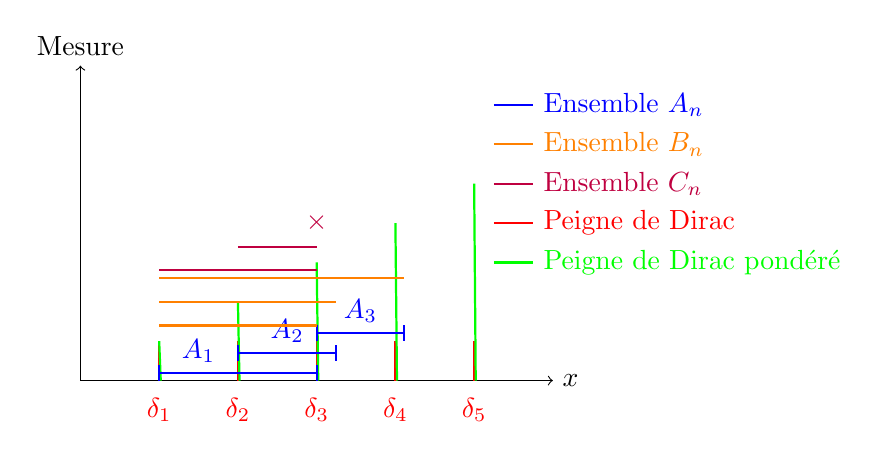
\begin{tikzpicture}
    % Axes
    \draw[->] (0,0) -- (6,0) node[right] {$x$};
    \draw[->] (0,0) -- (0,4) node[above] {Mesure};

    % Peigne de Dirac
    \foreach \x in {1,2,3,4,5} {
        \draw[red, thick] (\x,0) -- (\x,0.5);
        \draw[red] (\x,-0.1) node[below] {$\delta_{\x}$};
    }

    % Peigne de Dirac pondéré
    \foreach \x in {1,2,3,4,5} {
        \draw[green, thick] (\x+0.02,0) -- (\x,\x*0.5);
    }

    % Intervalles A_n
    \draw[blue, thick] (1.5,0.1) node[above] {$A_1$};
    % base line
    \draw[blue, thick] (1,0.1) -- (3,0.1);
    % edges
    \draw[blue, thick] (1,0.2) -- (1,0);
    \draw[blue, thick] (3,0.2) -- (3,0);


    \draw[blue, thick] (2,0.35) -- (3.25,0.35) node[midway, above] {$A_2$};
    % edges
    \draw[blue, thick] (2,0.45) -- (2,0.25);
    \draw[blue, thick] (3.25,0.45) -- (3.25,0.25);


    \draw[blue, thick] (3,0.6) -- (4.11,0.6) node[midway, above] {$A_3$};
    % edges
    \draw[blue, thick] (3,0.7) -- (3,0.5);
    \draw[blue, thick] (4.11,0.7) -- (4.11,0.5);

    % Intervalles B_n
    \draw[orange, thick] (1,0.7) -- (3,0.7);
    \draw[orange, thick] (1,1) -- (3.25,1);
    \draw[orange, thick] (1,1.3) -- (4.11,1.3);

    % Intervalles C_n
    \draw[purple, thick] (1,1.4) -- (3,1.4);
    \draw[purple, thick] (2,1.7) -- (3,1.7);
    \draw[purple] (3,2) node[circle] {$\times$};

    % Légende
    \draw[blue, thick] (5.25,3.5) -- (5.75,3.5) node[right] {Ensemble $A_n$};
    \draw[orange, thick] (5.25,3) -- (5.75,3) node[right] {Ensemble $B_n$};
    \draw[purple, thick] (5.25,2.5) -- (5.75,2.5) node[right] {Ensemble $C_n$};
    \draw[red, thick] (5.25,2) -- (5.75,2) node[right] {Peigne de Dirac};
    \draw[green, thick] (5.25,1.5) -- (5.75,1.5) node[right] {Peigne de Dirac pondéré};
\end{tikzpicture}
        \end{center}

        A partir du dessin, on peut facilement expliciter \(B_n\) et \(C_n\)
        pour déterminer que les mesures sont les suivantes:
        \begin{equation*}
            \begin{aligned}
                \mu(A_n)=2&\quad
                \nu(A_n)=2n+1&\quad
                \lambda(A_n)=1+\frac1n\\
                \mu(B_n)=n+1&\quad
                \nu(B_n)=\frac{(n+1)(n+2)}2&\quad
                \lambda(B_n)=n+\frac1n\\
                \mu(C_n)=0&\quad
                \nu(C_n)=0&\quad
                \lambda(C_n)=0
            \end{aligned}
        \end{equation*}
        Il est donc clair que pour \(n\) suffisament grand (pour se
        débarasser des cas particuliers), \(C_n\) tend vers le vide
        et \(B_n\) vers tout \(\N\).

        On pourrait expliciter les cas pour \(n\le 3\) mais cela a
        peu d'impact sur les résultats.
    \end{td-sol}
}{}

\begin{td-exo}[Mesure image]\, % 9
    
    Soient \((X,\scr A)\) et \((Y,\scr B)\) des espaces mesurables 
    et \(F:X\to Y\) une application mesurable. 
    
    Si \(\mu\) est une mesure sur \((X,\scr A)\), 
    on note \(F_*\mu:\scr B\to[0,+\infty]\) la mesure image de \(\mu\) par \(F\).
    \begin{enumerate}
        \item Pour \(a\in X\), déterminer \(F_*\delta_a\).
        \item On dit qu'une application \(G:\N\to \N\) préserve la mesure \(\chi\) si \(G_*\chi=\chi\).
        \begin{enumerate}
            \item Soit \(a\in\N\). À quelle condition l'application \(G\) préserve-t-elle la mesure \(\delta_a\)?
            \item À quelle condition l'application \(G\) préserve-t-elle la mesure de comptage?
        \end{enumerate}
    \end{enumerate}
\end{td-exo}
% --- sols

% 2.b => penser permutations/ bijections de \N dans \N
\begin{td-exo}
    Soit \((X,\scr A)\) un espace mesurable, \(\mu\) une mesure de probabilité sur \((X,\scr A)\), et soit \({(A_n)}_{n\in\N}\) une suite de parties mesurables telle que \(\forall n\in\N, \mu(A_n)=1\).
    \begin{enumerate} % 10
        \item    Montrer que \(\mu(\bigcap_{\in\N}A_n)=1\). Interpréter en passant au complémentaire.
        \item    Le résultat est-il encore vrai si on a \(\mu(X)=+\infty\)?
    \end{enumerate}
\end{td-exo}
% utiliser a_n=\N\setminus\{n\}, intersect nul, reste pas

\begin{td-exo}[Lois conditionnelles] % 11
    Soit \((\Omega,\scr F,\bb P)\) un espace probabilisé. Pour toute évènement \(A\in\scr F\) de probabilité non nulle, on considère l'application \(\bb P(\cdot|A):\scr F\to\R_+\) définie par \(\bb P(B|A)=\frac{\bb P(A\cap B)}{\bb P(A)}\).
    \begin{enumerate}
        \item Montrer que \(\bb P(\cdot|A)\) est une probabilité sur \((\Omega,\scr F)\).
        \item Pour tous évènements \(A,B\in\scr F\) de probabilités non nulles, exprimer \(\bb P(A|B)\) en fonction de \(\bb P(B|A)\), et en déduire la formule de Bayes.
    \end{enumerate}
\end{td-exo}
% ----- Solutions exo 11
\iftoggle{showsolutions}{
    \begin{td-sol}[]\,
        \begin{enumerate}
            \item Pour montrer que \(\bb P(\cdot|A)\) est une probabilité,
            il suffit de vérifier les axiomes d'une probabilité:
            \begin{itemize}
                \item On a \(\bb P(\varnothing|A)=\frac{\bb P(A\cap\varnothing)}{\bb P(A)}=0\).
                \item Soit \({(B_n)}_{n\in\N}\) une suite d'évènements disjoints. On a
                \begin{equation*}
                    \begin{aligned}
                        \bb P\left(\sqcup_{n\in\N}B_n|A\right)
                        &=\frac{\bb P\left(A\cap\left(\sqcup_{n\in\N}B_n\right)\right)}{\bb P(A)}\\
                        &=\frac{\bb P\left(\sqcup_{n\in\N}(A\cap B_n)\right)}{\bb P(A)}\\
                        &=\sum_{n\in\N}\frac{\bb P(A\cap B_n)}{\bb P(A)}\\
                        &=\sum_{n\in\N}\bb P(B_n|A).
                    \end{aligned}
                \end{equation*}
                \item On a \(\bb P(\Omega|A)=\frac{\bb P(A\cap\Omega)}{\bb P(A)}=1\).
            \end{itemize}
            \item On a
            \begin{equation*}
                \begin{aligned}
                    \bb P(A|B)
                    &=\frac{\bb P(A\cap B)}{\bb P(B)}\\
                    &=\frac{\bb P(B|A)\bb P(A)}{\bb P(B)}\\
                    &=\frac{\bb P(B|A)\bb P(A)}{\bb P(B|A)\bb P(A)+\bb P(B|A^C)\bb P(A^C)}\\
                    &=\frac{\bb P(B|A)\bb P(A)}{\bb P(B|A)\bb P(A)+\bb P(B|A^C)(1-\bb P(A))}.
                \end{aligned}
            \end{equation*}
            En posant \(C=A^C\), on obtient la formule de Bayes.
        \end{enumerate}
    \end{td-sol}
}{}

\begin{td-exo}[Fonctions de répartition] % 12
    Soit \((\Omega,\scr F,\bb P)\) un espace probabilisé et \(X:\Omega\to\R\) une variable aléatoire. La fonction de répartition de \(X\) est la fonction \(F_X:\R\to\R\) définie par \(F_X(t)=\bb P(X\le t)\).
    
    \begin{enumerate}
        \item Exprimer \(F_X\) à l'aide de la loi \(\bb P_X\) de \(X\). Que peut-on dire de la monotonie de \(F_X\)? Déterminer \(\displaystyle\lim_{t\to-\infty}F_X(t)\) et \(\displaystyle\lim_{t\to+\infty}F_X(t)\)
        
        \item Montrer \(F_X\) est continue à droite: pour tout \(a\in\R\) on a
        \(\displaystyle \lim_{\substack{t\to a \\ t>a}}F_X(t)=F_X(a)\).
        \item Montrer que \(F_X\) est continue sur \(\R\) si et seulement si \(\forall a\in\R\ \ \bb P(X=a)=0\).
    \end{enumerate}
\end{td-exo}
% ----- Solutions exo 12
\iftoggle{showsolutions}{
    \begin{td-sol}[]\,
        \begin{enumerate}
            \item On a
            \begin{equation*}
                F_X(t)=\bb P(X\le t)=\bb P_X(\of{-\infty,t}).
            \end{equation*}
            La fonction \(F_X\) est croissante car \(\bb P_X\) est une mesure de probabilité. On a
            \begin{equation*}
                \begin{aligned}
                    \lim_{t\to-\infty}F_X(t)
                    &=\lim_{t\to-\infty}\bb P_X(\of{-\infty,t})\\
                    &=\bb P_X(\varnothing)=0,\\
                    \lim_{t\to+\infty}F_X(t)
                    &=\lim_{t\to+\infty}\bb P_X(\of{-\infty,t})\\
                    &=\bb P_X(\R)=1.
                \end{aligned}
            \end{equation*}
            \item Soit \(a\in\R\). On a
            \begin{equation*}
                \begin{aligned}
                    \lim_{\substack{t\to a \\ t>a}}F_X(t)
                    &=\lim_{\substack{t\to a \\ t>a}}\bb P_X(\of{-\infty,t})\\
                    &=\bb P_X(\of{-\infty,a})\\
                    &=F_X(a).
                \end{aligned}
            \end{equation*}
            Pour rentrer la limite à droite, on utilise la continuité de la mesure de probabilité.
            Il est aussi possible d'utiliser la caractérisation séquentielle de la limite décroissante.

            Alors, par la proposition 2.24, on peut ecrire cet intervalle comme une intersection dénombrable d'intervalles ouverts.

            Comme \(F_X\) est croissante et bornée, on a bien la limite à gauche.

            \item Si \(F_X\) est continue sur \(\R\), alors pour tout \(a\in\R\), on a
            \begin{equation*}
                F_X(a)=\bb P_X(\of{-\infty,a})=\bb P_X(\oo{-\infty,a})=\bb P(X<a).
            \end{equation*}
            Donc \(\bb P(X=a)=0\). Réciproquement, si \(\bb P(X=a)=0\) pour tout \(a\in\R\), alors pour tout \(a\in\R\), on a
            \begin{equation*}
                F_X(a)=\bb P_X(\of{-\infty,a})=\bb P_X(\oo{-\infty,a})=\bb P(X<a).
            \end{equation*}
            Donc \(F_X\) est continue sur \(\R\).

            On peut en retenir que \(F_X\) est continue ssi 
            il n'y a pas de masses de Dirac dans la loi de \(X\).
            % idée: utiliser des suites croissantes pour montrer que la limite à droite est égale à la valeur en \(a\).
        \end{enumerate}
    \end{td-sol}
}{}

\begin{remark}
    La mesure de Lebesgue est invariante par translation. Réciproquement, cela permet de la caractériser.
\end{remark}

\begin{td-exo}[Invariance par translation de la mesure de Lebesgue]
    Soit \(a\in\R\) fixé. Pour tout \(A\subset\R\), on note \(A+a=\{x+a\ |\ x\in A\}\).
    \begin{enumerate}
        \item Montrer que \(A+a\in\scr B(\R)\) si et seulement si \(A\in\scr B(\R)\).
        \item pour tout \(A\in\scr B(\R)\), on note \(\mu(A)=\lambda_1(A+a)\), où \(\lambda_1\) est la mesure de Lebesgue sur \((\R,\scr B(\R))\). Montrer que l'application \(\mu\) ainsi définie est une mesure sur \((\R,\scr B(\R))\).
        \item Déduire de ce qui précède que la mesure de Lebesgue est invariante par translation: pour tout \(A\in\scr B(\R)\) on a \(\lambda_1(A+a)=\lambda_1(A)\).
    \end{enumerate}
\end{td-exo}
% ----- Solutions exo 13
\iftoggle{showsolutions}{
    \begin{td-sol}[]\,
        \begin{enumerate}
            \item Montrons que la famille des boréliens est stable par translation.
            Soit \(A\in\scr B(\R)\). On pose
            \begin{equation*}
                \begin{aligned}
                    \tau_a\colon \R&\to\R\\
                    x&\mapsto x+a
                \end{aligned}
            \end{equation*}
            Alors, on a
            \begin{equation*}
                \tau_a(A)=A+a=\tau_{-a}^{-1}(A).
            \end{equation*}
            Enfin,
            \begin{equation*}
                \tau_a^{-1}(A+a)=A
            \end{equation*}
            Si \(A\) est borélien, alors \(A+a\) est borélien. Réciproquement, si \(A+a\) est borélien, alors \(A\) est borélien.
            Donc la famille des boréliens est stable par translation.

            \item Montrons que \(\mu\) est une mesure.
            On utilise \(\tau_{-a}\) pour montrer que \(\mu\) est une mesure.

            On a alors
            \begin{equation*}
                \forall A\in\scr B(\R),\ \mu(A)={\left(\tau_{-a}\right)}_*\lambda_1(A)=\lambda_1(A+a).
            \end{equation*}
            Donc \(\mu\) est une mesure.

            \item Il suffit de montrer que \(\mu\) et \(\lambda_1\) coïncident sur les intervalles.
            Soit \(I=\oo{c,d}\) un intervalle. On a
            \begin{equation*}
                \begin{aligned}
                    \mu(I)&=\mu(\oo{c,d})\\
                    &=\lambda_1(\oo{c,d}+a)\\
                    &=\lambda_1(\oo{c+a,d+a})\\
                    &=d+a-(c+a)\\
                    &=d-c\\
                    &=\lambda_1(\oo{c,d})\\
                    &=\lambda_1(I).
                \end{aligned}
            \end{equation*}
            Alors \(\mu\) et \(\lambda_1\) coïncident sur les intervalles.

            Comme \(\lambda_1\) est invariante par translation, on a \(\mu=\lambda_1\).
        \end{enumerate}
    \end{td-sol}
}{}

\begin{td-exo}[Caractérisation de la mesure de Lebesgue]\label{exo_carac_lebesque}
    Pour tout intervalle \(I\subset\R\) et tout \(a\in\R\), on note \(I+a=\{x+a\ |\ x\in I\}\).
    
    Soit \(\mu\) une mesure sur \((\R,\scr B(\R))\) vérifiant les deux propriétés suivantes:
    \begin{itemize}
        \item \(\mu(\fo{0,1}) =1\);
        \item Pour tout intervalle \(I\subset\R\) et tout \(a\in\R\), on a \(\mu(I+a)=\mu(I)\).
    \end{itemize}
    Le but est de montrer que \(\mu\) est la mesure de Lebesgue.
    \begin{enumerate}
        \item Montrer \(\mu(\{x\})=0\) pour tout \(x\in\R\).\ \textit{On dit que la mesure \(\mu\) est diffuse.}
        \item Montrer que \(\mu(\fo{0,x})=x\) pour tout \(x\in\R_+^*\).\ \textit{On pourra commencer par le montrer pour tout rationnel \(x\in\bb Q_+^*\).}
        \item En déduire que \(\mu=\lambda_1\).
    \end{enumerate}
\end{td-exo}
% ----- Solutions exo 14
\iftoggle{showsolutions}{
    \begin{td-sol}[]\,
        \begin{enumerate}
            \item On a \(\{0\}=\bigcap_{n\in\N^*}\fo{0,\frac1n}\).
            Donc \(\mu(\{0\})=\lim_{n\to\infty}\mu\left(\fo{0,\frac1n}\right)=0\).
            Donc \(\mu(\{x\})=0\) pour tout \(x\in\R\) (à détailler).
            
            On écrira, pour \(I_n=\fo{0,\frac1n}\),
            \begin{equation*}
                \mu\left(\{0\}\right) = \mu\left(\bigcap_{n}^\infty I_n\right)
                =\lim_{n\to\infty}\mu\left(I_n\right)
                =\lim_{n\to\infty}\frac1n=0.
            \end{equation*}
            Comme on a \(\forall x\in\R\)
            \begin{equation*}
                \mu(\{x\})=\mu(\{0\}+x) = \mu(\{0\})=0,
            \end{equation*}
            on en déduit que \(\mu(\{x\})=0\) pour tout \(x\in\R\).

            \item Soit \(x\in\Q_+^*\), il existe \(k,n\in\N^\ast\) 
            tels que \(x=\frac{k}{n}\).
            On écrit alors
            \begin{equation*}
                \begin{aligned}
                    \mu\left(\fo{0,x}\right)
                    &=\mu\left(\fo{0,\frac{k}{n}}\right)\\
                    &=\mu\left(\bigsqcup_{i=0}^{n-1}\fo{0,\frac{1}{n}}+\frac{i}{n}\right)\\
                    &=\frac{k}{n}.
                \end{aligned}
            \end{equation*}
            On a montré que \(\mu(\fo{0,x})=x\) pour tout \(x\in\Q_+^*\).

            On prend maintenant \(x\in\R_+^*\). Alors, il existe une suite \({(x_n)}_{n\in\N^\ast}\subset\Q_+^*\) telle que \(x_n\to x\). Alors
            \begin{equation*}
                \begin{aligned}
                    \mu\left(\fo{0,x}\right)
                    &=\mu\left(\bigcup_{n=0}^{+\infty}\fo{0,x_n}\right)\\
                    &=\lim_{n\to\infty}\mu\left(\fo{0,x_n}\right)\\
                    &=\lim_{n\to\infty}x_n\\
                    &=x.
                \end{aligned}
            \end{equation*}
            Dans le cas pratique, cette suite correspond aux troncatures du développement décimal de \(x\).

            On a montré que \(\mu(\fo{0,x})=x\) pour tout \(x\in\R_+^*\).

            \item On conclut avec l'invariance par translation:

            Soient \(a,b\in\R\). Alors
            \begin{itemize}
                \item Si \(a=b\), voir question 1.
                \item Si \(a<b\), \(\mu(\oo{a,b})=\mu(\oo{0,b-a})=b-a\).
                \item Si \(a>b\), \(\mu(\oo{a,b})=\mu(\oo{b,a})=a-b\).
            \end{itemize}
            On a montré que \(\mu\) coïncide avec l'unique mesure qui satisfait les deux propriétés initiales.
            Donc \(\mu=\lambda_1\).
        \end{enumerate}

    \end{td-sol}
}{}

%
%===============================================================================
\subsection{Pour s'entrainer, pour aller plus loin} 
%===============================================================================
%

%

\begin{td-exo}
    Soit \(X=\{1,2,3,4,5,6\}\) et soit \(\scr C=\bigl\{\{1\},\{2,4\},\{2,5\}\bigr\}\subset\scr P(X)\). Déterminer \(\sigma(\scr C)\).
\end{td-exo}

\begin{td-exo}[Tribu image réciproque]
    Soit \(X\) un ensemble, \((Y,\scr B)\) un espace mesuré, et \(f:X\to Y\) un application. On note
    \[
        f^{-1}(\scr B)=\{f^{-1}(B)\ |\ B\in\scr B\}.
    \]
    \begin{enumerate}
        \item Montrer que \(f^{-1}(\scr B)\) est une tribu sur \(X\).
        \item On suppose que \(\scr A\) est une tribu sur \(X\). Montrer que \(f\) est \(\scr A\)-\(\scr B\)-mesurable si et seulement si \(f^*(\scr B)\subset\scr A\).
    \end{enumerate}
\end{td-exo}

\begin{td-exo}{}
    Soit \(\lambda_1\) la mesure de Lebesgue sur \(\R\), \(\delta_0\) la mesure de Dirac en \(0\), et \(\mu=\lambda_1+\delta_0\).
        \begin{enumerate}
            \item Calculer \(\mu(\bigcap_{n\ge 1}A_n)\), où \(A_n=\fo{0,\frac{1}{n}}\);
            \item Calculer \(\mu(\bigcup_{n\ge 1}A_n)\), où \(A_n=\fo{\frac{1}{n},1}\);
            \item Calculer \(\mu(\bigcup_{n\ge 1}A_n)\), où \(A_n=\fo{-\frac{1}{n},2-\frac{1}{n}}\);
            \item Calculer \(\mu(\bigcap_{n\ge 1}A_n)\), où \(A_n=\ff{-\frac{1}{n},1-\frac{1}{n}}\).
        \end{enumerate}
\end{td-exo}

%

\begin{td-exo}
    Soit \(A\in\scr B(\R^n)\) tel que \(\lambda_n(A)=0\). Montrer que \(A\) est d'intérieur vide.
\end{td-exo}

\begin{td-exo}[Extrait d'un sujet d'examen.]
    
    Soit \((X,\scr A)\) un espace mesurable, où \(\scr A\) est une tribu qui contient les singletons. Dans ce qui suit, toutes les mesures considérées sont des mesures sur \((X,\scr A)\).
    
    On dit qu'une mesure \(\mu\) est \emph{diffuse} si elle vérifie \(\forall x\in X\ \ \mu(\{x\})=0\).
    
    On dit qu'une mesure \(\mu\) est \emph{discrète} s'il existe une partie dénombrable \(D\subset X\) telle que \(\mu(D^c)=0\).
    
    \begin{enumerate}
        \item Montrer qu'une mesure \(\mu\) est diffuse si et seulement si, pour toute partie dénombrable \(A\subset X\) on a \(\mu(A)=0\).
        
        \item Soit \(\mu\) une mesure discrète, et soit \(D\subset X\) dénombrable tel que \(\mu(D^c)=0\). Montrer qu'il existe des réels positifs \({(\alpha_a)}_{a\in D}\) tels que \(\displaystyle \mu=\sum_{a\in D}\alpha_a\delta_{a}\).
        
        \item Soit \(\mu\) une mesure finie, et soit \(D=\bigl\{x\in X\ |\ \mu(\{x\})>0\bigr\}\).
        \begin{enumerate}
            \item Pour tout \(n\in\N^*\) on note \(E_n=\bigl\{x\in X\ |\ \mu(\{x\})>\frac{1}{n}\bigr\}\). Montrer que \(E_n\) est une partie finie de \(X\) pour tout \(n\in\N^*\) et en déduire que \(D\) est dénombrable.
            \item Pour tout \(A\in\scr A\) on note \(\nu(A)=\mu(A\cap D^c)\). Montrer que \(\nu\) est une mesure diffuse.
            \item Montrer que \(\mu\) est la somme d'une mesure diffuse et d'une mesure discrète.
        \end{enumerate}
        
        \item Montrer que le résultat de la question 3.\ (c) est encore vrai si la mesure \(\mu\) est \(\sigma\)-finie.
    \end{enumerate}
\end{td-exo}
    

%
\begin{td-exo}[Un exemple de partie non mesurable]
    
    On considère la relation d'équivalence sur \(\ff{0,1}\) définie par
    \[
    x\sim y\ \Longleftrightarrow x-y\in\bb Q.
    \]
    On peut donc écrire \(\ff{0,1}\) comme l'union disjointe de ses classes d'équivalences: \(\displaystyle\ff{0,1} = \bigsqcup_{i\in I}C_i\).
    
    Pour tout \(i\in I\) on se donne un élément \(x_i\in C_i\) et on considère \(A=\{x_i\ |\ i\in I\}\). Par ailleurs, pour tout \(q\in\bb Q\cap\ff{-1,1}\), on note \(A_q=A+q\).
    \begin{enumerate}
        \item Montrer que \(A_q\cap A_r = \varnothing\) si \(q\neq r\).
        
        \item Montrer que \(\displaystyle \ff{0,1} \subset \bigcup_{q\in\bb Q\cap\ff{-1,1}}A_q \subset \ff{-1,2}\).
        
        \item En supposant que \(A\) est borélien, exprimer \(\lambda_1(\bigcup_{q\in\bb Q\cap\ff{-1,1}}A_q)\) en fonction de \(\lambda_1(A)\). Conclure.
    \end{enumerate}
\end{td-exo}